% Final report, Proyek Akhir NLP Gasal 2026: extractive MRC (Indonesian, SQuAD v2 style).
% Render: python miscellaneous/scripts/render_latex.py report/latex/main.tex report/main.pdf
% Paths are relative to this folder. Generated tables and figures are pulled in directly, so rerunning the
% analysis updates the report: cross-model -> ../assets/, EDA -> ../../eda/outputs/, per experiment ->
% ../../experiments/NN-*/analysis/. Lines marked TODO are for the team to write.
\documentclass[11pt,a4paper]{article}
\usepackage[utf8]{inputenc}
\usepackage[T1]{fontenc}
\usepackage[margin=2.5cm]{geometry}
\usepackage{amsmath}
\usepackage{graphicx}
\usepackage{booktabs}
\usepackage{xcolor}
\usepackage{colortbl}
\usepackage{pdflscape}
\usepackage{longtable}
% light tints per error category (error-analysis tables)
\definecolor{ecorrect}{HTML}{C8E6C9}
\definecolor{elong}{HTML}{FFE0B2}
\definecolor{eshort}{HTML}{FFF9C4}
\definecolor{ewsent}{HTML}{C5CAE9}
\definecolor{ewspan}{HTML}{E1BEE7}
\definecolor{enoans}{HTML}{FFCDD2}
\usepackage[numbers]{natbib}
\usepackage[hidelinks]{hyperref}
% \usepackage[indonesian]{babel}  % uncomment for an Indonesian report

% Laporan ini bisa ditreat sbg log dan penemuan eksperimen kita seiring berjalan. Jadi, ketika kita nyoba model X, motivasinya, yang dituangkan ke dalam sutdi literatur, eda, error analysis, itu berkesinambungan dair perocbaan model sebelumnya yang sudah ada di laporan ini. Jadi, -- at least gw --  gw prefernya nyobain model itu hasilnya paralel buat studi ltieratur hingga error analysis etika dituangkan ke laporan.

% Sebagai contoh, gw (atau siapapun nanti) pegnen nunukkin dari hasil EDA kata-kata mana yang ada di pertanyaan tetapi gaada di konteks. Ada kata pada pertanyaan yang mangarahkan ke jawabannya (siapa PEMIMPIN vs PRESIDEN Indonesia) tapi kata eksaknya ada gaada di korpus. Ada juga kata-kata yang agak jauh dan kurang bisa menjadi sinonim antara kata di pertnayana sama kotneks, misalnya nanya "BERAPA", tentunya di konteks ngga ada kata yang bersinonim layaknya "presiden" dengna "pemimpin", paling-paling adanya "jumlah penduduk Indonesia adalah ..." secara tidak langsung. Ini buat motivasi kenapa ngga make rule base dan kenapa harus make embedding, perhaps bukan embedding biasa tapi juga harus make attention mechanism biarrelasi yang lebih kompeks kayak pertanyaan "berapa" dengan teks yg menyatakan kuantitias di teks konteks itu bisa ketangkep. Kemudian, dari hasil implementasi word embedding atau trasnformer, tulis error analysisnay dan jadikan ini motivasi buat perkemabngan selanjutnya.

\graphicspath{{../assets/figures/}{../../eda/outputs/figures/}}
\newcommand{\todo}[1]{\textcolor{red}{[TODO: #1]}}
\newcommand{\expdir}[1]{\texttt{experiments/#1}}

\title{Extractive Machine Reading Comprehension for Indonesian:\\
Classical Pipeline, BiDAF, IndoBERT and LLMs}
\author{Muhammad Aldo Fahrezy \\
Naufal Zafran Fadil \\
Fernando Lawrence}
\date{\today}

\begin{document}
\maketitle

\begin{abstract}
\todo{Task, data (Indonesian Wikipedia passages, 44\% unanswerable), the models, the headline result
(IndoBERT 73.5 F1 on our dev split) and the main error-analysis finding.}
\end{abstract}

\section{Introduction}
\todo{Task definition (span extraction or abstain, SQuAD v2 \citep{rajpurkar2018know}), why answerability is the
hard part, and the contributions.}

\subsection{Definisi Task}

Secara umum, merujuk pada ~\cite{Zeng2020}, MRC pada tugas ini merupakan MRC dengan tipe pertanyaan 'Natural', yaitu berupa kalimat pertanyaan yang sahih secara grammar bahasa Indonesia, serta bertipe jawaban 'Span', yaitu jawabannya merupakan bagian dari teks konteks. Adapun definisi task dari MRC pada tugas ini adalah:

Diberikan konteks $C = \{c_0, \dots, c_k, \dots, c_{lc}\}$, pertanyaan $Q = \{q_0, \dots, q_j, \dots, q_{lq}\}$ dan jawaban $A = \{c_m, \dots, c_n\}$, dengan $lc$ dan $lq$ merepresentasikan panjang (atau banyak kata) pada konteks dan pertanyaan, $c_k$ dan $q_j$ merupakan kata dalam \textit{vocabulary} atau bisa dinotasikan sebagai $c_k, q_j \in V$, $C$ dan $Q$ membentuk teks yang mematuhi grammar alami bahasa Indonesia, serta $0 \leq m \leq n \leq lc$. Kita ingin membuat model $\mathcal{M}$ sedemikian sehingga $\mathcal{M}(C, Q) = A$ untuk setiap pasangan $(C, Q, A)$ pada dataset.


\section{Studi Literatur}

\subsection{Dataset dan Leaderboard}

~\cite{Zeng2020} menjabarkan beberapa data \textit{open source} beserta taksonomi jenis-jenisnya. Berhubung data MRC pad atugas ini berupa pertanyaan 'Natural' dan jawaban 'Span', ada beberapa dataset yang dapat menjadi refernsi dan perbandingan hasil atau EDA seperti pada Gambar~\ref{fig:zeng_taxonomy}. Selain itu, kami menggunakan \textit{leaderboard} yang dipublikasikan oleh dataset tersebut sebagai target dan inspirasi untuk epngembangan model kami. Sebagai contoh, pada \textit{leaderboard} SQuAD2.0 \footnote{https://rajpurkar.github.io/SQuAD-explorer/}, terlihat bahwa \textit{human-level performance} (HLP) memiliki EM $86{,}831$ dan F1 $89{.}452$ dan terdapat $30$ model yang berhasil melampaui HLP. Hal ini bisa menjadi target \textit{upper-bound} hasil model kami serta inspirasi untuk memperbaiki error pada model kami. Beberapa di antara model yang melampaui HLP sering kali memakai model yang sama seperti ALBERTA dan ELECTRA dan peringkat $10$ teratas \textit{leaderboard} merupakan \textit{ensemble}.

\begin{figure}[t]
  \centering
  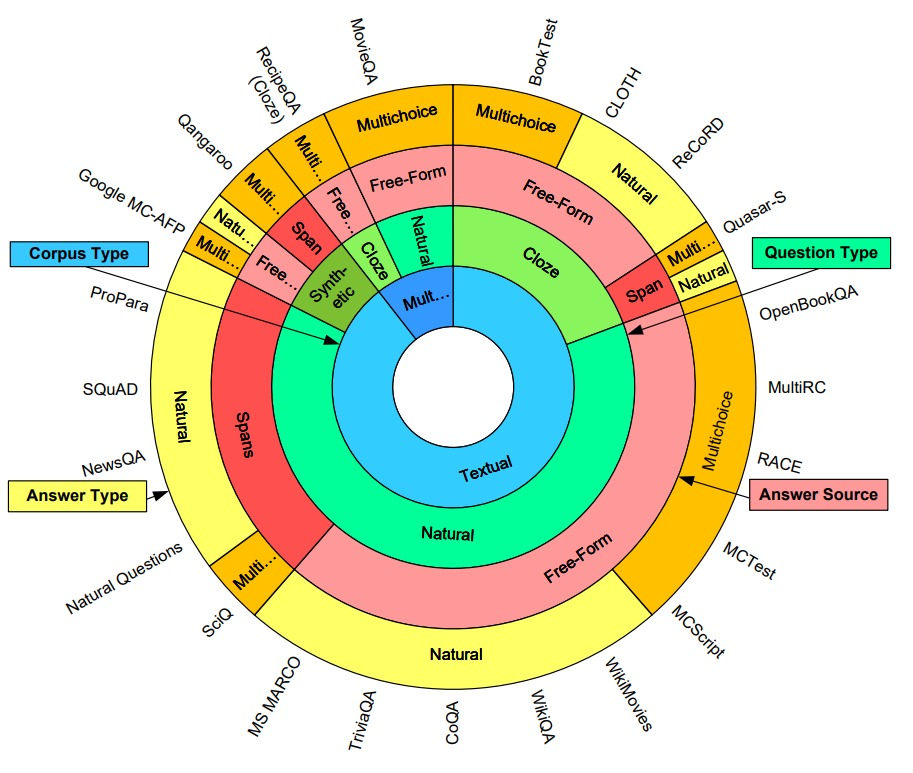
\includegraphics[width=\linewidth]{Zeng2020_dataset_taxonomy.jpeg}
  \caption{Taksonomi dataset MRC \textit{open source} menurut \cite{Zeng2020}.}
  \label{fig:zeng_taxonomy}
\end{figure}

\todo{\begin{itemize}
\item coba cari literatur juga terkait pengaruh pergantian bahasa (FT BERT jadi IndoBERT) ke pengaruh model beserta error pointsnya. Mungkin juga refer ke paper yg datanya ada culture2nya, kita-kira weakpointnya di mana dan dibanding sm error analysis kita gimana, sama suggested improvements serta limitasi mereka di mana.
\end{itemize}}

\subseciton{Bahasa dan Penalaran Model}

\paragraph{Kemampuan pemahaman model dalam \textit{task} multilngual.} \cite{Liu2026} menyugesti bahwa \textit{large reasoning models} memiliki pemahaman multilingual yang bias terhadap bahasa yang \textit{high-resource}, terlebih lagi bahasa Ingriss dan bahasa-bahasa yang satu rumpun (Jerman, Belanda, dll.). \cite{Tezuka2025} menunjukkan bahwa ada sekumpulan neuron yang berfungsi untuk mentranslasikan berbagai bahasa dari input menjadi representasi laten untuk \textit{reasoning} model kemudian terdapat sekumpulan neuron pula yang mentranslasikan dari representasi laten ke bahasa tujuan. Mereka menunjukkan bahwa terdapat sekumpulan neuron yang berbeda untuk setiap bahasa dalam mengenali fitur linguistik bahasa tersebut.

Hal ini memotivasi kami untuk mengeksplorasi metode lain dalam menginkorporasi dan melatih model berbahasa Indonesia selain melalui melalui \textit{fine-tuning} secara penuh yang sering kali membuthukan banyak sumber daya untuk berhasil. Salah satu contohnya adalah seperti yang diusulkan \cite{Yoon2024}, yaitu menambahkan multilingual \textit{encoder} untuk 'menyelaraskan' berbagai macam bahasa ke representasi laten yang digunakan oleh LLM. Namun begitu, kami perlu melakukan \textit{error analysis} terkait untuk mengarahkan dan menjustifikasi keputusan teknis yang akan diambil.

\subsection{Model}

\subsubsection{Famili BERT}

\paragraph{ALBERT \cite{Lan2019}.} Sebagai salah satu model dengan performa teratas pada \textit{leaderboard}, ALBERT memberikan beberapa pembaruan dari BERT, di antaranya:

\begin{itemize}
  \item Faktorisasi parameter embedding.  \cite{Lan2019} berargumen bahwa dimensi \textit{context-dependent embedding} seharusnya lebih besar dari \textit{context-independent embedding} sebab \textit{context-dependent embedding} memuat lebih banyak informasi. Namun, memiliki \textit{embedding table} sebesar $|V| \times |H|$ dengan $H$ adalah dimensi \textit{context-dependent embedding} sangat boros, sehingga \cite{Lan2019} menggunakan parameter tambahan untuk memproyeksikan \textit{context-dependent embedding table} ke \textit{context-independent embedding table}.
  \item \textit{Cross-layer parameter sharing}. ALBERT melakukan \textit{parameter sharing} pada setiap layernya sebagai \textit{default}.
  \item  \textit{Sentence-order prediction} (SOP) sebagai pengganti \textit{loss/task} NSP. \cite{Lan2019} berargumen bahwa \textit{NSP} yang digunakan dalam \textit{pre-training} mencampurkan \textit{task topic prediction} \textit{coherence prediction}, padahal \textit{topic prediction} pada NSP jauh lebih mudah dari \textit{coherence predction} dan bercampur juga dengan \textit{loss} yang dimodelkan oleh \textit{loss} MLM. Oleh karena itu \cite{Lan2019} menggunakan SOP yang menguji model untuk memprediksi apakah dua pasang kalimat memiliki urutan yang asli atau si-\textit{swap}. 
\end{itemize}

\subsubsection{Perkembangan Lanjut}

\cite{Zhang2020} menambahkan metode baru di atas ALBERT dan ELECTRA dengan membuat model dapat melakukan 'skimming' dan '\textit{intensive reading}' layaknya manusia membaca atau menyelesaikan \textit{task} MRC ini dan mendapatkan nilai EM dan F1 sebesar 90{.}578	dan 92{.}978 berturut-turut. 

Banyaknya literatur dan perkembangan model yang berangkat dari ALBERT dan ELECTRA memotivasi kami untuk mencoba kedua model ini beserta membangun metode selanjutnya di atas model ini. 

\section{Data and exploratory analysis}
\label{sec:data}
% Source: eda/README.md, miscellaneous/docs/data_card.md, eda/outputs/
\todo{Split (grouped by passage: 6435/803/804 train/dev/internal test), passage, question and answer
statistics, answer types and positions.}

\begin{figure}[t]
  \centering
  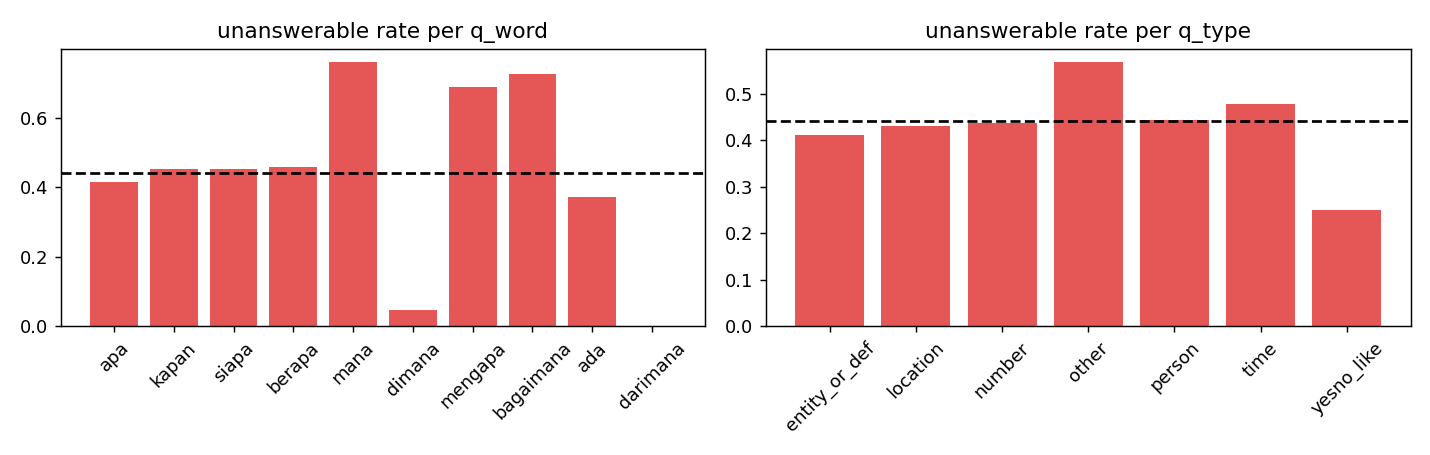
\includegraphics[width=0.8\linewidth]{eda_unanswerable_rate.png}
  \caption{Share of unanswerable questions. \todo{interpretation}}
  \label{fig:unans}
\end{figure}

\paragraph{Dataset artifacts.} \todo{A question-only classifier predicts answerability with AUC 0.90
(eda/outputs/tables/artifact\_probe.json); unanswerable questions are minimal edits of answerable ones.}

\section{Models}
\label{sec:models}
% Each model maps to one experiment folder; its summary.md has architecture, input and prediction details.
\subsection{Baselines (\expdir{01-baseline-trivial})}
Always no-answer, and a sliding-window baseline \citep{richardson2013mctest}.
\subsection{Classical pipeline with feature engineering (\expdir{02-classical-pipeline-lgbm})}
\todo{Three stages: answerability (LightGBM \citep{ke2017lightgbm}), sentence retrieval (TF-IDF, BM25
\citep{robertson2009probabilistic}, logistic regression), span ranking (LightGBM lambdarank). Features.}
\subsection{BiDAF (\expdir{03-nn-bidaf})}
\todo{BiDAF-lite \citep{seo2017bidirectional} trained from scratch with a NULL position; the no-attention ablation.}
\subsection{Pretrained encoder (\expdir{04-plm-indobert})}
\todo{IndoBERT-base-p1 \citep{wilie2020indonlu}, BERT-style QA head \citep{devlin2019bert}, sliding windows,
no-answer score.}
\subsection{Large language models (\expdir{05-llm-local-qwen}, \expdir{06-llm-api-offtheshelf})}
\todo{Prompting, parsing and grounding to a passage span; local models and off-the-shelf API models.}

\section{Experimental setup}
\todo{Metrics (EM, F1, HasAns F1, NoAns accuracy), the no-answer threshold tuned on dev (dev-optimistic),
3 seeds, paired bootstrap for significance, hardware.}

\section{Results}
\begin{table}[t]
  \centering
  \small
  \begin{tabular}{lrrrrrl}
\toprule
Model & Seeds & EM & F1 & HasAns F1 & NoAns acc & F1 95\% CI \\
\midrule
no\_answer & 1 & 46.20 $\pm$ 0.00 & 46.20 $\pm$ 0.00 & 0.00 $\pm$ 0.00 & 100.00 $\pm$ 0.00 & [42.59, 49.44] \\
sliding\_window & 1 & 46.20 $\pm$ 0.00 & 46.20 $\pm$ 0.00 & 0.00 $\pm$ 0.00 & 100.00 $\pm$ 0.00 & [42.84, 49.69] \\
sliding\_window\_thr & 1 & 46.08 $\pm$ 0.00 & 46.81 $\pm$ 0.00 & 4.37 $\pm$ 0.00 & 96.23 $\pm$ 0.00 & [43.07, 50.25] \\
classical\_pipeline & 3 & 50.98 $\pm$ 0.23 & 53.36 $\pm$ 0.21 & 29.13 $\pm$ 1.14 & 81.58 $\pm$ 1.34 & [49.98, 56.49] \\
bidaf\_noattn & 3 & 52.47 $\pm$ 0.66 & 56.47 $\pm$ 0.56 & 30.66 $\pm$ 1.29 & 86.52 $\pm$ 2.17 & [53.43, 59.52] \\
bidaf & 3 & 52.68 $\pm$ 0.73 & 56.61 $\pm$ 0.72 & 28.15 $\pm$ 3.20 & 89.76 $\pm$ 3.42 & [53.56, 59.74] \\
plm\_indobert\_full & 3 & 69.45 $\pm$ 0.46 & 73.55 $\pm$ 0.43 & 59.16 $\pm$ 1.25 & 90.30 $\pm$ 0.79 & [70.82, 76.29] \\
\bottomrule
\end{tabular}

  \caption{Dev results, mean $\pm$ std over seeds; the no-answer threshold is tuned on dev.
  Generated by \texttt{mrc.analysis.compare}.}
  \label{tab:main}
\end{table}
\todo{Discuss table~\ref{tab:main} and the significance tests (report/assets/tables/significance.md).}

\begin{figure}[t]
  \centering
  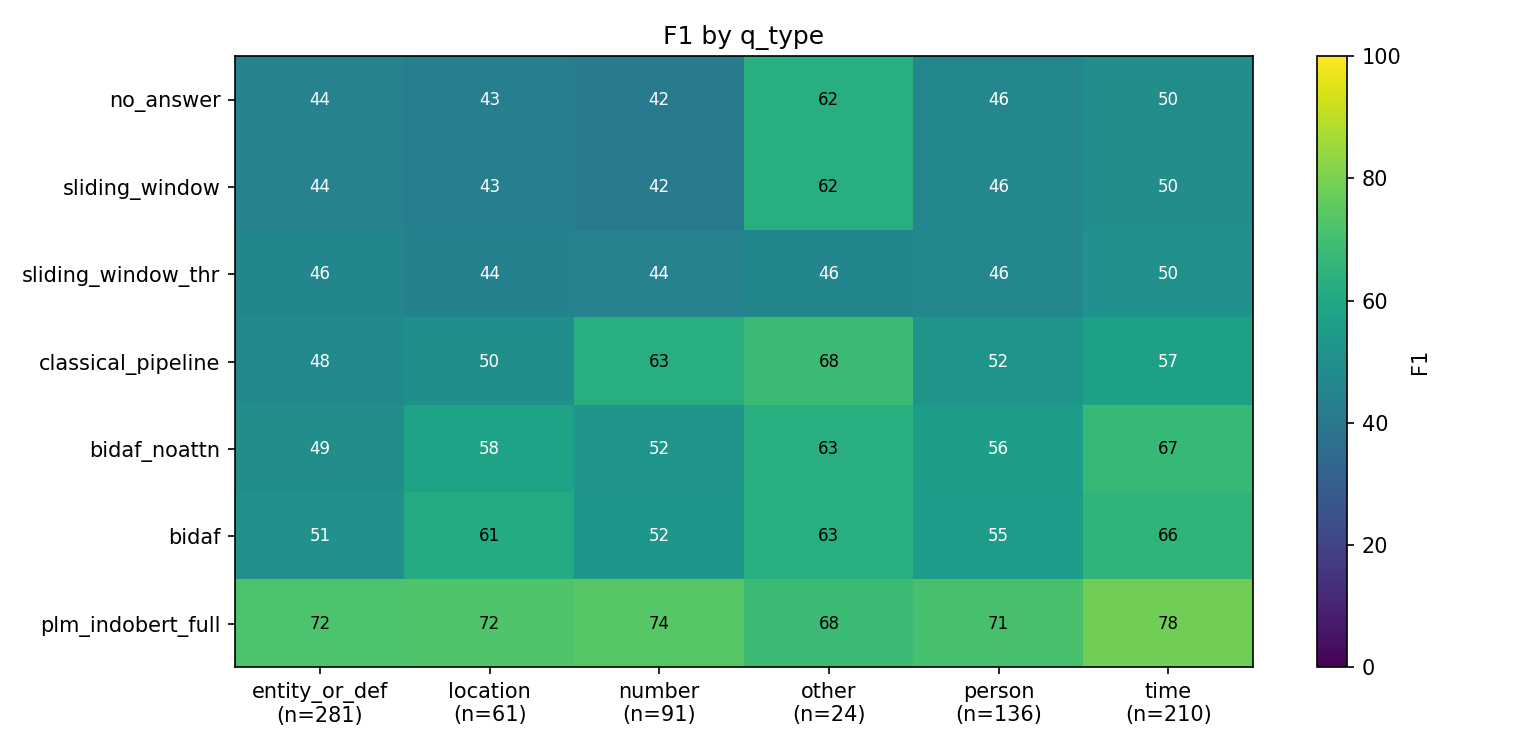
\includegraphics[width=\linewidth]{heatmap_q_type.png}
  \caption{F1 by question type. \todo{interpretation}}
  \label{fig:qtype}
\end{figure}

\section{Error analysis}
% Per experiment: experiments/NN-*/analysis/ (outcomes, slices, error samples for manual labels).
% Across models: eda/notebooks/model_errors.ipynb and report/assets/tables/.
% Definitions mirror classify() in experiments/global/mrc/analysis/compare.py.
\textbf{Definisi jenis error.}
Misalkan $A$ adalah jawaban acuan (gold) dan $\hat{A} = \mathcal{M}(C, Q)$ jawaban model, keduanya berupa \textit{span}
$\{c_m, \dots, c_n\}$ pada konteks $C$ atau himpunan kosong $\emptyset$ bila tidak ada jawaban. Misalkan
$\tau(\cdot)$ adalah deret token setelah normalisasi (huruf kecil, tanpa tanda baca dan penanda sitasi seperti \texttt{[1]}) dan $G = \tau(A)$,
$P = \tau(\hat{A})$. Bila terdapat beberapa gold, dipakai gold dengan F1 tertinggi terhadap $\hat{A}$. Notasi
$X \sqsubseteq Y$ berarti $X$ adalah sub-deret kontigu dari $Y$, dan $s(\cdot)$ adalah indeks kalimat pada $C$ yang memuat
awal \textit{span}. Setiap jawaban salah ($\mathrm{EM}(\hat{A}, A) = 0$) diklasifikasikan ke tepat satu jenis berikut,
diperiksa berurutan. (1)~\textit{False answer on unanswerable}: $A = \emptyset$ tetapi $P \neq \emptyset$, yaitu model menjawab pada
pertanyaan yang tidak dapat dijawab. (2)~\textit{False no answer}: $A \neq \emptyset$ tetapi $P = \emptyset$, yaitu model
abstain padahal jawaban ada. Selanjutnya, untuk $G \neq \emptyset$ dan $P \neq \emptyset$:
(3)~\textit{Boundary too long}: $G \sqsubseteq P$ dan $G \neq P$, yaitu jawaban model memuat seluruh gold ditambah token berlebih;
(4)~\textit{Boundary too short}: $P \sqsubseteq G$ dan $P \neq G$, yaitu jawaban model hanya sebagian dari gold;
(5)~\textit{Partial overlap}: $\mathrm{F1}(P, G) > 0$ tetapi tidak berlaku (3) maupun (4);
(6)~\textit{Wrong span, same sentence}: $\mathrm{F1}(P, G) = 0$ dan $s(\hat{A}) = s(A)$, yaitu \textit{span} salah pada kalimat yang benar;
(7)~\textit{Wrong sentence}: $\mathrm{F1}(P, G) = 0$ dan $s(\hat{A}) \neq s(A)$, yaitu \textit{span} berasal dari kalimat lain.
Jawaban dengan $\mathrm{EM} = 1$ disebut \textit{correct}. Dalam kode, jenis ini tertulis sebagai \texttt{false\_answer\_on\_unanswerable},
\texttt{false\_no\_answer}, \texttt{boundary\_too\_long}, \texttt{boundary\_too\_short}, \texttt{partial\_overlap},
\texttt{wrong\_span\_same\_sentence}, dan \texttt{wrong\_sentence}.

\begin{figure}[t]
  \centering
  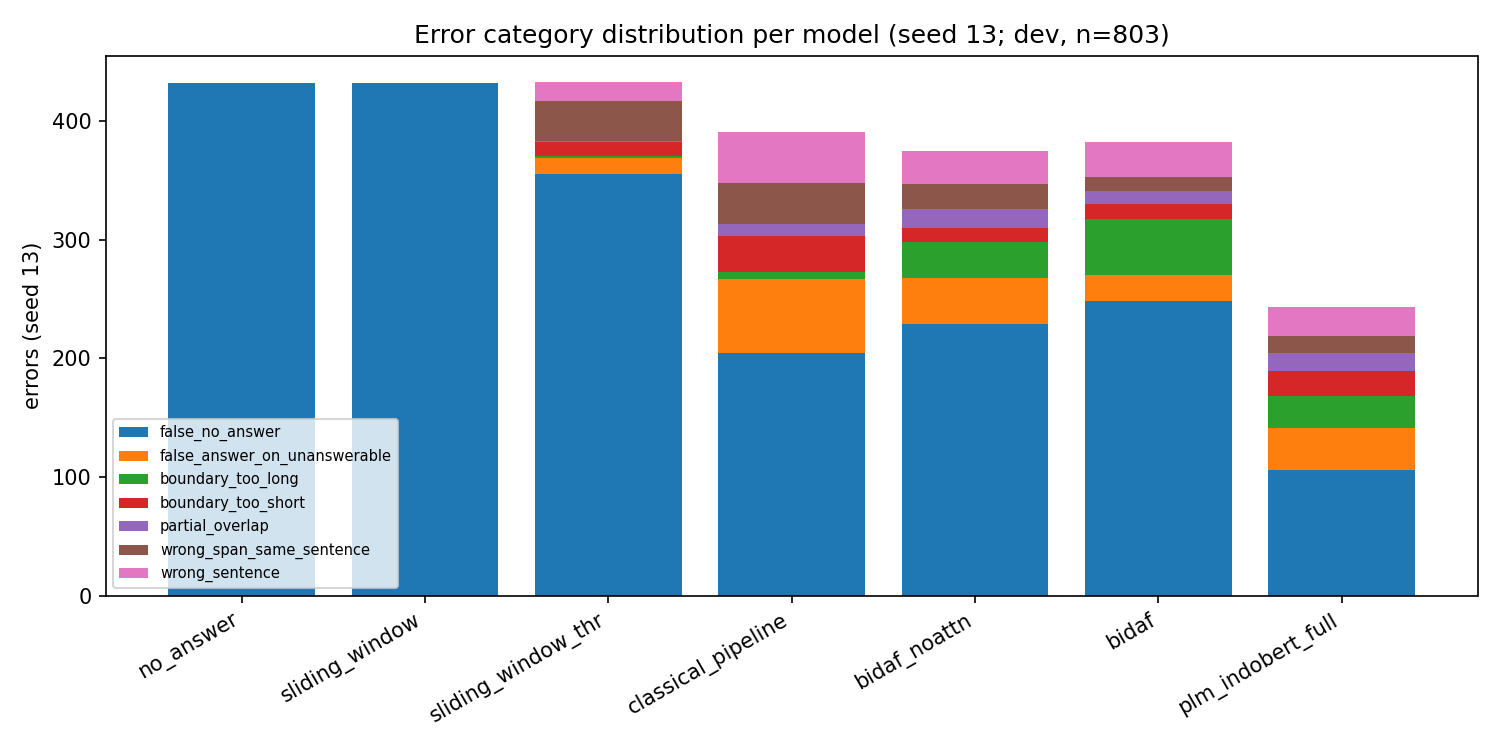
\includegraphics[width=\linewidth]{error_taxonomy_stacked.png}
  \caption{Error types per model (seed 13). \todo{interpretation}}
  \label{fig:errors}
\end{figure}
\subsection{Analisis berdasarkan contoh jawaban model}
\label{sec:ea-examples}
Tabel~\ref{tab:examples} pada Lampiran~\ref{app:examples} membandingkan jawaban setiap model (seed 13) pada contoh dev
yang dijawab oleh seluruh model utama, lengkap dengan konteksnya, dan dikelompokkan ke dalam empat sekat sesuai penyebab
error-nya. Warna sel menunjukkan jenis error sehingga pola antarmodel mudah dibandingkan.

\paragraph{Lebih dari satu jawaban valid.}
Pada pertanyaan ``Dimana letak Düsseldorf?'', gold-nya hanya \textit{Jerman}, padahal kalimat kedua pada konteks juga
menjawab pertanyaan yang sama secara valid (\textit{tepi Sungai Rhein}). Hampir semua model, yaitu \textit{classical
pipeline}, IndoBERT, Nemotron, dan Gemini, memilih jawaban kedua dan dihitung sebagai \texttt{wrong\_sentence} dengan
F1 $0$, sedangkan BiDAF hanya memperoleh kredit parsial (F1 $0{,}50$ untuk \textit{Jerman bagian Barat}). Error ini
lebih mencerminkan keterbatasan anotasi dengan satu jawaban acuan daripada kegagalan pemahaman model, sehingga EM dan F1
menghukum jawaban yang sebenarnya dapat diterima.

\paragraph{Inkonsistensi ekspektasi jawaban.}
Konteks Papua yang sama muncul dengan dua pertanyaan yang hampir identik, tetapi gold-nya berbeda: \texttt{808.105km}
pada ``Berapa luas Papua?'' dan \texttt{808.105km persegi} pada ``berapakah luas Papua?''. Seluruh model, termasuk
Nemotron, selalu menjawab \textit{808.105km persegi}. Akibatnya jawaban yang sama dianggap \texttt{boundary\_too\_long}
(F1 $0{,}67$) pada kasus pertama dan benar sepenuhnya pada kasus kedua. Pada contoh Kanada dan Gorontalo, gold juga
memuat satuan (\textit{kilometer persegi}, \textit{km$^2$}) sehingga seluruh model benar. Pola ini menunjukkan bahwa
model mempelajari konvensi ``angka beserta satuannya'', dan error batas pada kasus Papua pertama merupakan
inkonsistensi anotasi, bukan kesalahan model.

\paragraph{Tanda baca konteks yang ambigu.}
Pada ``apakah nama ibukota Afganistan?'', konteks hanya berbunyi ``Di samping ibu kotanya Kabul, Herat, Jalalabad,
Mazar-e Sharif dan Kandahar ialah kota-kota utama negara ini''. Koma yang sama memisahkan apositif (\textit{Kabul}) dan
daftar kota lain sehingga batas jawaban tidak terlihat dari tanda bacanya. Hanya \textit{classical pipeline} yang
menjawab benar (\textit{Kabul}); BiDAF-noattn memilih daftar kota tanpa \textit{Kabul} (\texttt{wrong\_span\_same\_sentence}),
sedangkan BiDAF dan IndoBERT memperpanjang \textit{span} hingga seluruh daftar (\texttt{boundary\_too\_long}).

\paragraph{Konteks berupa daftar tanpa penanda jabatan.}
Pada ``Siapa presiden pertama Nauru?'', konteks adalah tabel yang terflatten menjadi daftar nama dan tanggal
(``NamaMasa jabatan 1.\ Hammer DeRoburt (1922-1992) 31 Januari 1968 -- \ldots{}'') tanpa satu pun kata \textit{presiden}
atau keterangan jabatan lain yang menunjukkan siapa mereka. Model harus menyimpulkan bahwa nama pertama pada daftar adalah
presiden pertama. Akibatnya \textit{classical pipeline}, BiDAF-noattn, IndoBERT, dan Gemini memilih tidak menjawab
(\texttt{false\_no\_answer}), BiDAF memilih judul kolom \textit{NamaMasa jabatan1} (\texttt{wrong\_sentence}), dan hanya
Nemotron yang menjawab mendekati benar (\textit{Hammer DeRoburt (1922-1992)}, F1 $0{,}80$). Ini contoh kasus yang
memerlukan penalaran struktur dokumen, bukan pencocokan leksikal antara pertanyaan dan konteks.

\subsection{Analisis error Qwen2.5-14B-Instruct \textit{few-shot} pada \textit{official validation}}
\label{sec:ea-qwen14b}
% Sumber: experiments/07-llm-offtheshelf-fewshot/runs/official_val/Qwen2.5-14B-Instruct_fs_id/ (report_official_val.md)
% dan experiments/07-llm-offtheshelf-fewshot/analysis/official_val/. IndoBERT memakai threshold yang di-tune pada dev.
Qwen2.5-14B-Instruct (4-bit, prompt \texttt{fs\_id} dengan 7 demo, \textit{greedy decoding}) dijalankan pada 1000
pertanyaan pertama dari urutan tetap \textit{official validation}, yaitu 640 pertanyaan \textit{answerable} dan 360
\textit{unanswerable}. Keputusan menjawab atau abstain diambil langsung dari keluaran model tanpa \textit{threshold}.
Pada 1000 pertanyaan yang sama, Qwen memperoleh EM $63{,}0$ dan F1 $75{,}1$, sedangkan IndoBERT dengan
\textit{threshold} dari dev memperoleh EM $61{,}9$ dan F1 $68{,}6$ (rata-rata tiga \textit{seed}). Selisih F1 yang jauh
lebih besar daripada selisih EM menunjukkan bahwa Qwen sering menemukan bagian konteks yang benar, tetapi jarang
memotong \textit{span} tepat seperti gold. \textit{Threshold} yang di-tune langsung pada data ini hanya menaikkan EM Qwen
menjadi $63{,}8$, sehingga ruang perbaikan utama tidak berada pada \textit{threshold}.

Tabel~\ref{tab:qwen-outcomes} membandingkan jenis error kedua model. Kedua model gagal dengan cara yang berlawanan.
Qwen unggul pada pertanyaan \textit{answerable} (EM $51{,}9$ dibanding $46{,}4$ untuk IndoBERT \textit{seed} 13), tetapi
kalah pada pertanyaan \textit{unanswerable} (akurasi $82{,}8$ dibanding $88{,}1$). Kesalahan memilih kalimat
(\texttt{wrong\_sentence}) turun dari 57 pada IndoBERT menjadi 17 pada Qwen. Sebaliknya, \texttt{boundary\_too\_long}
naik dari 63 menjadi 128 dan menjadi jenis error terbesar Qwen.

\begin{table}[t]
  \centering
  \caption{Jenis jawaban pada 1000 pertanyaan pertama \textit{official validation}. IndoBERT memakai \textit{seed} 13
  dengan \textit{threshold} dari dev; Qwen memakai keputusan apa adanya.}
  \label{tab:qwen-outcomes}
  \begin{tabular}{lrr}
    \toprule
    Jenis & Qwen2.5-14B & IndoBERT \\
    \midrule
    \texttt{correct\_ans} & 332 & 297 \\
    \texttt{correct\_no\_ans} & 298 & 317 \\
    \texttt{boundary\_too\_long} & 128 & 63 \\
    \texttt{false\_no\_answer} & 87 & 113 \\
    \texttt{false\_answer\_on\_unanswerable} & 62 & 43 \\
    \texttt{boundary\_too\_short} & 31 & 46 \\
    \texttt{partial\_overlap} & 30 & 28 \\
    \texttt{wrong\_sentence} & 17 & 57 \\
    \texttt{wrong\_span\_same\_sentence} & 15 & 36 \\
    \bottomrule
  \end{tabular}
\end{table}

\paragraph{Batas \textit{span} terlalu panjang.}
Error \texttt{boundary\_too\_long} menyumbang $12{,}8$ dari $37{,}0$ poin EM yang hilang, tetapi hanya $4{,}4$ dari
$24{,}9$ poin F1. Hal ini karena tambahannya pendek: median gold 3 token, median prediksi 7 token, dan median token berlebih
2. Pada 67 dari 128 kasus, kelebihannya hanya berada di depan gold. Kata yang ditambahkan umumnya penanda takrif atau
keterangan, misalnya \textit{suatu satuan dasar materi} (gold \textit{satuan dasar materi}), \textit{para pedagang Arab},
\textit{bahasa Yunani Koine}, \textit{bulan Mei 1940}, dan \textit{Di sekitar tahun 1994}. Kelebihan di belakang gold
biasanya berupa keterangan dalam kurung atau klausa lanjutan, misalnya \textit{3.062 delegasi dengan hak suara dan 158
tanpa hak suara} untuk gold \textit{3.062}. Qwen menjawab dengan frasa yang lengkap secara gramatikal, sedangkan konvensi
anotasi dataset ini memilih inti jawaban. Konvensi tersebut terlihat pada data latih: kurang dari $0{,}4\%$ gold
\textit{answerable} di train diawali \textit{suatu}, \textit{sebuah}, \textit{seorang}, \textit{para}, \textit{di},
\textit{pada}, atau \textit{sekitar}. Membuang kata-kata tersebut dari awal jawaban Qwen menaikkan EM dari $63{,}0$
menjadi $64{,}3$. Kelemahan ini juga menjelaskan rendahnya EM Qwen pada pertanyaan lokasi ($48$ dibanding $63$ untuk
IndoBERT), karena 24 dari 101 pertanyaan lokasi berakhir sebagai \texttt{boundary\_too\_long}.

\paragraph{Keputusan abstain.}
Skor \textit{no-answer} Qwen, yaitu selisih \textit{log-probability} antara jawaban dan \texttt{unanswerable}, membedakan pertanyaan \textit{answerable} dan
\textit{unanswerable} sedikit lebih buruk daripada IndoBERT (AUC $0{,}898$ dibanding $0{,}935$). Pemeriksaan manual
terhadap 16 sampel acak \texttt{false\_\allowbreak no\_\allowbreak answer} menunjukkan bahwa sebagian besar abstain tersebut tidak sepenuhnya
salah. Enam kasus memiliki gold yang tidak menjawab pertanyaan. Contohnya, gold untuk ``Kapan John meninggal?'' adalah
tanggal kremasi, gold untuk ``Siapakah pendiri maskapai Air Asia?'' adalah pemilik awalnya, dan konteks untuk ``apakah
ras kucing terkecil didunia?'' tidak menyebut ukuran sama sekali. Lima kasus lain ambigu karena entitas di pertanyaan dan
konteks berbeda tipis, misalnya desa dan kecamatan Karangkancana. Hanya lima kasus yang merupakan kegagalan model:
tiga kasus memerlukan pencocokan alias atau ejaan nama (``Kaisar Yuan'' dan \textit{Yuan Shikai}), satu kasus memerlukan
relasi terbalik (``isteri'' dari frasa \textit{suami Fofo Fauzia}), dan satu kasus seharusnya terjawab langsung.

Pada 16 sampel acak \texttt{false\_answer\_on\_unanswerable}, tujuh kasus muncul karena Qwen mengabaikan
pewatas di pertanyaan, seperti \textit{menurut ensiklopedia}, \textit{menurut ahli}, \textit{mata uang logam}, dan
\textit{Taekwondo yang modern}. Dua kasus mengandung negasi (``Siapa yang bukan bagian dari grup Guns N' Roses?''), tiga
kasus dijawab dengan pengetahuan di luar konteks (misalnya \textit{Jumong} sebagai raja pertama Goguryeo, padahal
konteks hanya menyebut ia mengungsi), dan empat kasus sebenarnya dapat dijawab dari konteks, misalnya tahun runtuhnya
Dinasti Ming. Pola pewatas dan negasi ini sama dengan jebakan \textit{unanswerable} yang diuraikan pada taksonomi error.
Delapan dari 615 jawaban Qwen tidak ditemukan di konteks, termasuk satu jawaban yang memuat komentar model.

\paragraph{Komplementaritas dengan IndoBERT.}
Kedua model benar pada sekitar 474 pertanyaan, hanya Qwen yang benar pada sekitar 156, dan hanya IndoBERT yang benar pada
sekitar 145, sehingga \textit{oracle} yang selalu memilih model yang benar mencapai EM $77{,}5$. Dua aturan sederhana
tanpa parameter memanfaatkan pola ini. Aturan pertama memakai \textit{span} IndoBERT jika \textit{span} tersebut berada
di dalam jawaban Qwen, sehingga batas yang terlalu panjang terpotong. Aturan ini menaikkan EM menjadi $66{,}5$--$66{,}7$
untuk ketiga \textit{seed} IndoBERT. Aturan kedua menambahkan keputusan ``jawab jika salah satu model menjawab'' dan
mencapai EM $67{,}4$--$67{,}5$ serta F1 $76{,}6$--$77{,}0$. Kedua aturan dipilih setelah melihat data ini, sehingga
angkanya masih optimistis dan perlu diuji pada 1003 pertanyaan \textit{official validation} lainnya sebelum dipakai
untuk leaderboard.

\todo{Correct and wrong examples, strengths and weaknesses of each model, error causes, reasoning challenges
(manual labels from the error samples).}

\section{Discussion and conclusion}
\todo{What worked, limits (dev-tuned thresholds, partial LLM API runs), future work.}

\appendix
\begin{landscape}
\section{Contoh jawaban model}
\label{app:examples}
{\scriptsize
\setlength{\tabcolsep}{3pt}
\renewcommand{\arraystretch}{1.25}
\begin{longtable}{p{2.0cm}p{1.6cm}p{5.2cm}p{1.9cm}p{1.9cm}p{1.9cm}p{1.9cm}p{2.1cm}p{2.1cm}}
  \caption{Jawaban setiap model pada contoh dev yang dijawab oleh semua model utama (seed 13), dibahas pada
  Subbab~\ref{sec:ea-examples}. Teks tebal pada konteks adalah jawaban gold. Warna sel menunjukkan jenis error:
  \colorbox{ecorrect}{benar}, \colorbox{elong}{batas terlalu panjang}, \colorbox{ewsent}{kalimat salah},
  \colorbox{ewspan}{span salah pada kalimat yang sama}, \colorbox{enoans}{tidak menjawab}. ``--'' berarti model API tidak
  dijalankan pada contoh tersebut.}
  \label{tab:examples} \\
    \toprule
    Pertanyaan & Gold & Konteks & Classical & BiDAF-noattn & BiDAF & IndoBERT & Nemotron (API) & Gemini (API) \\
    \midrule
    \endfirsthead
    \multicolumn{9}{l}{\textit{Tabel~\ref{tab:examples} (lanjutan)}} \\
    \toprule
    Pertanyaan & Gold & Konteks & Classical & BiDAF-noattn & BiDAF & IndoBERT & Nemotron (API) & Gemini (API) \\
    \midrule
    \endhead
    \midrule
    \multicolumn{9}{r}{\textit{berlanjut di halaman berikutnya}} \\
    \endfoot
    \bottomrule
    \endlastfoot
    \multicolumn{9}{l}{\cellcolor{black!8}\textit{Lebih dari satu jawaban valid}} \\*
    Dimana letak Düsseldorf? & Jerman
      & Düsseldorf adalah ibu kota Negara Bagian Nordrhein-Westfalen di \textbf{Jerman} dan (bersama-sama dengan Köln dan Wilayah Ruhr) merupakan pusat ekonomi Jerman bagian Barat. Düsseldorf terletak di tepi Sungai Rhein dan merupakan salah satu pusat utama dari daerah Rhein-Ruhr \ldots
      & \cellcolor{ewsent}Sungai Rhein
      & \cellcolor{elong}pusat ekonomi Jerman bagian Barat
      & \cellcolor{elong}Jerman bagian Barat
      & \cellcolor{ewsent}tepi Sungai Rhein
      & \cellcolor{ewsent}Düsseldorf terletak di tepi Sungai Rhein
      & \cellcolor{ewsent}tepi Sungai Rhein \\
    \midrule
    \multicolumn{9}{l}{\cellcolor{black!8}\textit{Inkonsistensi ekspektasi jawaban}} \\*
    Berapa luas Papua? & 808.105km
      & \ldots{} Papua memiliki luas \textbf{808.105km} persegi dan merupakan pulau terbesar kedua di dunia dan terbesar pertama di Indonesia.
      & \cellcolor{elong}808.105km persegi & \cellcolor{elong}808.105km persegi & \cellcolor{elong}808.105km persegi
      & \cellcolor{elong}808.105km persegi & \cellcolor{elong}808.105km persegi & -- \\
    berapakah luas Papua? & 808.105km persegi
      & (Konteks sama:) \ldots{} Papua memiliki luas \textbf{808.105km persegi} dan merupakan pulau terbesar kedua di dunia \ldots
      & \cellcolor{ecorrect}808.105km persegi & \cellcolor{ecorrect}808.105km persegi & \cellcolor{ecorrect}808.105km persegi
      & \cellcolor{ecorrect}808.105km persegi & -- & -- \\
    berapakah luas Kanada? & 9.970.610 kilometer persegi
      & \ldots{} Kanada merupakan negara terluas di Amerika Utara. Luas negara Kanada adalah \textbf{9.970.610 kilometer persegi}. Kanada digolongkan negara maju \ldots
      & \cellcolor{ecorrect}9.970.610 kilometer persegi & \cellcolor{ecorrect}9.970.610 kilometer persegi
      & \cellcolor{ecorrect}9.970.610 kilometer persegi & \cellcolor{ecorrect}9.970.610 kilometer persegi & -- & -- \\
    Berapa luas provinsi Gorontalo? & 12.435,00km$^2$
      & Provinsi Gorontalo terletak pada Semenanjung Gorontalo di Pulau Sulawesi \ldots{} Luas wilayah provinsi ini \textbf{12.435,00km$^2$} dengan jumlah penduduk sebanyak 1.133.237 jiwa (2016) \ldots
      & \cellcolor{ecorrect}12.435,00km$^2$ & \cellcolor{ecorrect}12.435,00km$^2$ & \cellcolor{ecorrect}12.435,00km$^2$
      & \cellcolor{ecorrect}12.435,00km$^2$ & -- & -- \\
    \midrule
    \multicolumn{9}{l}{\cellcolor{black!8}\textit{Tanda baca konteks yang ambigu}} \\*
    apakah nama ibukota Afganistan? & Kabul
      & Di samping ibu kotanya \textbf{Kabul}, Herat, Jalalabad, Mazar-e Sharif dan Kandahar ialah kota-kota utama negara ini. Lihat juga Kota-kota di Afganistan.
      & \cellcolor{ecorrect}Kabul
      & \cellcolor{ewspan}Herat, Jalalabad, Mazar-e Sharif dan Kandahar ialah kota-kota utama negara ini
      & \cellcolor{elong}Kabul, Herat, Jalalabad, \ldots{} Lihat juga Kota-kota di Afganistan
      & \cellcolor{elong}Kabul, Herat, Jalalabad, Mazar-e Sharif dan Kandahar & -- & -- \\
    \midrule
    \multicolumn{9}{l}{\cellcolor{black!8}\textit{Konteks berupa daftar tanpa penanda jabatan}} \\*
    Siapa presiden pertama Nauru? & Hammer DeRoburt
      & NamaMasa jabatan 1.\ \textbf{Hammer DeRoburt} (1922-1992) 31 Januari 1968 -- 22 Desember 1976 2.\ Bernard Dowiyogo (1946-2003) 22 Desember 1976 -- 19 April 1978 3.\ Lagumot Harris (1938-1999) \ldots{} 30.\ Baron Waqa (1959-) 11 Juni 2013 -- Sekarang
      & \cellcolor{enoans}(tidak menjawab) & \cellcolor{enoans}(tidak menjawab)
      & \cellcolor{ewsent}NamaMasa jabatan1 & \cellcolor{enoans}(tidak menjawab)
      & \cellcolor{elong}Hammer DeRoburt (1922-1992) & \cellcolor{enoans}(tidak menjawab) \\
\end{longtable}
}
\end{landscape}
\section{External resources}
\todo{Pretrained models, libraries and data used (miscellaneous/docs/decisions.md).}
\section{AI use declaration}
\todo{Which AI tools were used, for what, and how the output was checked.}

\bibliographystyle{plainnat}
\bibliography{references}
\end{document}
